\section{Controle de versão}

\begin{frame}
\frametitle{Git - sistema de controle de versão}

\begin{itemize}
\item Sistema de controle de versão distribuído.
\item Desenvolvido por Linus Torvalds para o desenvolvimento do kernel do Linux.
\item Repositório contendo códigos, textos, imagens, planilhas, etc.
\item Histórico de versões.
\item Acompanhamento de mudanças.
\item Ramificações (branches) e mesclas (merges).
\end{itemize}
\end{frame}

\begin{frame}
\frametitle{Git - reposotórios}

\begin{figure}[h]
\centering
\includegraphics[width=0.6\textwidth,height=0.6\textheight,keepaspectratio]{figures/git-push.png}
\caption{Repositório local e remoto. Fonte \url{https://www.javatpoint.com/git-push}}
\label{fig-git-push}
\end{figure}

\end{frame}
\note{
Um repositório é o local para armazenar os dados 
relativos a um determinado projeto. É importante 
mantê-lo organizado e documentado. O repositório
poderá ser utilizado por diversos usuários no
desenvolvimento distribuído do projeto. 

Cada usuário do repositório terá a sua cópia local
dos dados.

O usuário deve
1. buscar novas atualizações no repositório remoto,
2. fazer suas modificações locais,
3. submetê-las para o repositório.

\begin{itemize}
\item Os repositórios podem ser públicos ou privados.
\item Repositórios públicos são acessíveis a qualquer um, 
basta para tanto ter a URL deste repositório.
\item O repositório pertence a um usuário ou à uma equipe.
\item Apenas o dono do repositório (ou o administrador, no 
caso de uma equipe) poderá apagar o repositório.
\item O código de um projeto pode consistir apenas dos dados
contidos em um único repositório, ou pode ser uma combinação
de múltiplos repositórios, mesmo que sejam de diferentes assinaturas 
(ou proprietários).
\end{itemize}
}

\begin{frame}
\frametitle{Git - hospedagem}
\begin{itemize}
\item GitHub
\item Bitbucket
\item SourceForge
\item Google Developers
\item GNU Savannah
\item GitLab
\item hospedagem local
\item outros
\end{itemize}

\vspace{2ex}
obs: OverLeaf utiliza git
\end{frame}



\begin{frame}
\frametitle{Esquema git}
\begin{figure}[h]
\centering
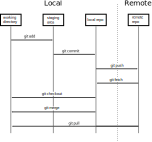
\includegraphics[width=0.8\textwidth,height=0.75\textheight,keepaspectratio]{figures/git-schema.pdf}
\caption{Esquema básico de utilização do git.}
\label{fig-git-schema}
\end{figure}
\end{frame}


\begin{frame}[fragile]
\frametitle{Criando um repositório local}
Inicialmente um repositório é vazio, mesmo que você
crie um repositório onde já existam arquivos.
Os arquivos deverão ser posteriormente adicionados 
ao repositório.

\begin{lstlisting}[language=bash, label=lst-git-repo, caption={Passos para criar um repositório local no Linux.}, postbreak=\mbox{$\hookrightarrow$\space}, basicstyle=\fontsize{8}{10}\selectfont\ttfamily]
# muda do diretorio corrente para o diretorio do repositorio
$ cd ~/myrepo
# inicializa o repositorio local
$ git init
# adiciona um arquivo e deixa-o pronto para o commit 
#               (perpetrar, alocar)
$ git add filename
# ou
# adiciona os arquivos no diretorio corrente
$ git add .
# realiza o commit dos aquivos preparados
$ git commit -m "mensagem de commit"
\end{lstlisting}
\end{frame}

\begin{frame}[fragile]
\frametitle{Repositório remoto}

\begin{lstlisting}[language=bash, label=lst-git-repo2, caption={Adicionando um repositório remoto.}, postbreak=\mbox{$\hookrightarrow$\space}, basicstyle=\fontsize{8}{10}\selectfont\ttfamily]
# adiciona o repositorio remoto
$ git remote add origin URL_do_repositiorio
# verificacao
$ git remote -v
# envia as modificacoes para o repositorio remoto
$ git push origin master
\end{lstlisting}
\end{frame}

\begin{frame}[fragile]
\frametitle{Clonando um repositório}
\begin{lstlisting}[language=bash, label=lst-git-repo2, caption={Clonando um repositório.}, postbreak=\mbox{$\hookrightarrow$\space}, basicstyle=\fontsize{8}{10}\selectfont\ttfamily]
$ git clone https://url_do_repositorio
# ou
$ git clone https://url_do_repositorio outro_nome
# caso queira dar outro nome ao diretorio
\end{lstlisting}

Será criado um diretório com o nome do repositório, inicializa-se o arquivo .git
e baixa todo o conteúdo do repositório.
\end{frame}


\begin{frame}[fragile]
\frametitle{Comandos básicos}

\begin{itemize}
\item \verb|git pull|
\item \verb|git status|
\item \verb|git add nome_do_arquivo|
\item \verb|git rm nome_do_arquivo|
\item \verb|git commit -m 'message'|
\item \verb|git push origin master|
\item \verb|git comando --help|
\end{itemize}

\end{frame}

\begin{frame}[fragile]
\frametitle{Configurações do repositório ou globais}
\begin{lstlisting}[language=bash, label=lst-git-conf1, caption={Configurações do git.}, postbreak=\mbox{$\hookrightarrow$\space}, basicstyle=\fontsize{8}{10}\selectfont\ttfamily]
# informar seu usuario
$ git config --global user.name "nome_do_usuario"
# --global: For writing options: write to global ~/.gitconfig file rather than the repository .git/config
$ git config --local user.name "nome_do_usuario"
# --local: For writing options: write to the repository .git/config file.
# verificar as informacoes
$ git config --global --list 
$ git config --list 
\end{lstlisting}
\end{frame}


\begin{frame}[fragile]
\frametitle{Chave SSH}
Utilizando chave SSH não é necessário digitar login e senha a cada utilização do repositório remoto.
\begin{lstlisting}[language=bash, label=lst-git-ssh, caption={Utilização de chave SSH.}, postbreak=\mbox{$\hookrightarrow$\space}, basicstyle=\fontsize{8}{10}\selectfont\ttfamily]
# verifique se existe ja criou uma chave
$ ls -al ~/.ssh
# um dos arquivos: id_rsa.pub, id_ecdsa.pub ou id_ed25519.pub
# para criar uma chave
$ ssh-keygen -t ed25519 -C "email@ufsj.edu.br"
# para adicionar a chave a um agente
$ eval "$(ssh-agent -s)"
$ ssh-add ~/.ssh/id_ed25519
# gerando uma nova chave
$ ssh-keygen -t ed25519-sk -C "email@ufsj.edu.br"
\end{lstlisting}

leia mais:
\url{https://docs.github.com/en/github/authenticating-to-github/connecting-to-github-with-ssh}
\end{frame}


\begin{frame}[fragile,allowframebreaks]
\frametitle{Iniciando um repositório}
\begin{lstlisting}[language=bash, label=lst-git-init, caption={Inicializando um repositório.}, postbreak=\mbox{$\hookrightarrow$\space}, basicstyle=\fontsize{8}{10}\selectfont\ttfamily]
$ git init # inicializar um repositorio
$ touch README.md # criar um arquivo README
$ git add . # adiciona todos os arquivos ao repositorio
$ git add README.md # adiciona apenas o arquvio README
$ git status # verifica o status do repositorio (novos, modificados e commited)
$ git commit -m "mensagem sobre este commit" # mensagens sao uteis
$ git remote add origin URL_do_repositorio_remoto # configura o repositorio remoto
$ git remote -v # lista as coneccoes remotas
$ git push origin master # envias as modificacoes 
# GitHub passou a utilizar `main' como nome do repositorio remoto, mas podemos trocar
$ git fetch # traz os arquivos do repositorio remoto para o repositorio local
$ git merge # junta as modificacoes do repositorio local ao diretorio de trabalho
$ git pull # usado para buscar os arquivos atualizados do repositorio remoto
# git pull equivale a: git fetch + git merge
\end{lstlisting}
\end{frame}

\begin{frame}[fragile]
\frametitle{Ignorando certos arquivos}
O arquivo \texttt{.gitignore} é utilizado para listar os arquvos que o git deve ignorar.

\begin{lstlisting}[language=bash, label=lst-git-ignore, caption={Exemplo de arquivo \texttt{.gitignore}.}, postbreak=\mbox{$\hookrightarrow$\space}, basicstyle=\fontsize{8}{10}\selectfont\ttfamily]
*.log
*.aux
*.bbl
*.bcf
*.out
errs.txt
article*.bmp
\end{lstlisting}
\end{frame}


\begin{frame}[fragile,allowframebreaks]
\frametitle{Verificando as mudanças}
\begin{lstlisting}[language=bash, label=lst-git-diff, caption={Analisando as mudanças realizadas.}, postbreak=\mbox{$\hookrightarrow$\space}, basicstyle=\fontsize{8}{10}\selectfont\ttfamily]
$ git diff # mostras os arquivos modificados
$ git diff --name-only # mostra apenas os nomes
$ git diff --name-status # nomes e status
$ git diff --color-words # diferencas palavra-por-palavra (colorido)
$ git diff --color-words HEAD^ HEAD arquivo # diferenca da versao atual com o commit anterior
# podemos utilziar ^ ou ~1 (um representa quando commits atrás)
$ git diff --color-words HEAD^ HEAD nome_do_arquivo | ansi2html > /tmp/diff.html # gerar um relatio em HTML
\end{lstlisting}

\framebreak

\begin{lstlisting}[language=bash, label=lst-git-log, caption={Log das alterações.}, postbreak=\mbox{$\hookrightarrow$\space}, basicstyle=\fontsize{8}{10}\selectfont\ttfamily]
$ git log # verificar o historico de commits
$ git log --since="1 hour ago" -- _filename_ # historico da ultima hora para um arquivo
$ git log --follow -- _filename_ # listar todos commits que modificaram um arquivo
$ git log --pretty=format: --name-only --since="1 hour ago" | sort | grep .tex | uniq # para listar todos os arquivos que foram modificados na ultima hora
\end{lstlisting}

\framebreak

\begin{lstlisting}[language=bash, label=lst-git-diff2, caption={Script para gerar um relatório das mudanças nas últimas horas em arquivos \texttt{.tex}.}, postbreak=\mbox{$\hookrightarrow$\space}, basicstyle=\fontsize{8}{10}\selectfont\ttfamily]
SWHEN="12 hour ago"
git log --pretty=format: --name-only --since="$SWHEN" | sort | grep .tex | uniq |
while read FILENAME
do
  echo $FILENAME
  PCOMMIT=$(git log --since="$SWHEN" -- $FILENAME | grep commit | sed 's/commit //g' | tail -n 1)
  COMMIT=$(git log  --follow -- $FILENAME | grep commit | sed 's/commit //g' | sed -e "1,/$PCOMMIT/d" | head -n 1)
  git diff --color --word-diff $COMMIT HEAD -- $FILENAME
done | ansi2html > /tmp/diff.html
\end{lstlisting}
\end{frame}





\begin{frame}
Sugestões de leitura: 
\vspace{2ex}

\fullcite{chacon_pro_2014}
\url{https://git-scm.com/book/en/v2}

\vspace{3ex}
\href{https://www.youtube.com/watch?v=xEKo29OWILE&list=PLHz_AreHm4dm7ZULPAmadvNhH6vk9oNZA}{Curso de Git e GitHub (Gustavo Guanabara)}

\end{frame}


